\chapter{Discussion}\label{chap:discussion}
In this chapter, we will discuss the results obtained from our intrinsic (Section~\ref{sec:discussion_intrinsic}) and extrinsic (Section~\ref{sec:discussion_extrinsic}) evaluations. We will discuss the performance of our models and the overall system. Additionally, we aim to address the limitations and challenges encountered during the evaluation process (Section~\ref{sec:discussion_limitations}).\\
We will assess whether the models we employed and the overall BiBEx system can effectively address our research questions. We aim to determine if the system we developed is robust and unified, capable of accurately extracting metadata from document headers and references, irrespective of the language in which they are written, be it English or German.

\section{Intrinsic Evaluation}\label{sec:discussion_intrinsic}
% document segmentation
As evident in Table~\ref{tab:results_document_segment_compare}, our experiments show that our fine-tuned LayoutXLM model achieved the best results in almost all categories, except in the figure class. This may seem counterintuitive, since the LayoutXLM architecture explicitly envelops visual information and figures should be one of the most striking features in a document.\\
We believe that this is the result of the different creation processes of our self-annotated dataset and the DocBank dataset. Figures in the DocBank dataset are assigned the token '\textit{\#\#LTFigure\#\#}' and '\textit{\#\#LTLine\#\#}' with bounding boxes enclosing the entire figure. As we can see in Table~\ref{tab:results_docseg_lang}, the LayoutXLM model is capable to nearly perfectly predict figure labels of the DocBank portion of the dataset.\\
OCR systems on the other hand usually do not extract illustrations as a whole and instead try to distil text from these images. This can result in artefacts, where the OCR system detects non-existing text or text fragments in figures. Due to our premise to create a robust dataset, we decided to keep these artefacts and label them as figures. We believe that these artefacts can stand out in a coherent text, which is why text-based classifiers can accurately predict them.\par
We observed also fairly high F1-scores for the '\textit{reference}' class of all employed models with only the CRF model performing worse than the rest. However, our results suggest that visual information might not be the predominant feature to detect reference sections in articles, since both mBERT and XLM-RoBERTa show good results, relying only on textual information.\\
On the other hand show classes we are predominately interested in, namely author, abstract, and title considerable improvements against their reference models. These classes typically protrude in articles, for example are title often written in a bigger font or abstracts highlighted in bold. This suggests, that the visual information fed into LayoutXLM indeed seems to facilitate the models ability to correctly predict its classes.\\

\begin{figure}[!ht]
    \centering
    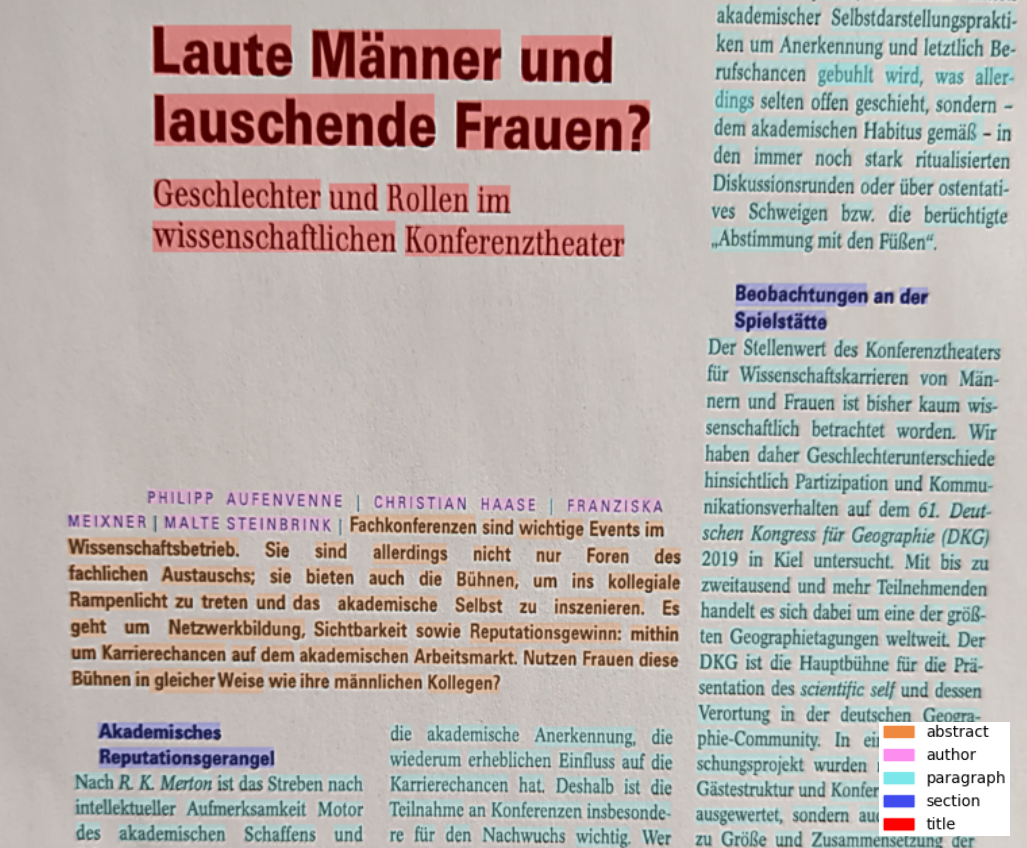
\includegraphics[width=0.85\linewidth]{images/layoutxlm.png}
    \caption{The detected classes of an article by our fine-tuned LayoutXLM model. Despite the faulty layout caused by the OCR process, as depicted in Figure~\ref{fig:layout_error}, we are able to extract all authors.}
    \label{fig:layoutxlm_result}
\end{figure}

The confusion matrix depicted in Figure~\ref{fig:results_final_docseg_conf} shows a slight bias for some labels towards the majority class '\textit{paragraph}'. In many cases these errors occurred in articles, where text segments of a certain class are unusually long, for example long abstracts or footer sections. LayoutXLM is further constricted by the amount of maximum token it can predict, which can remove contextual information surrounding long sections. All of this hinders the correct classification of long text sections for certain classes.\\
Furthermore, we noticed that documents with less discriminating visual features, as shown for example in Figure~\ref{fig:no_seperation}, where we have no clear separation between abstract and the following text section, are prone to have higher error rates.\\
\begin{figure}[!t]
    \centering
    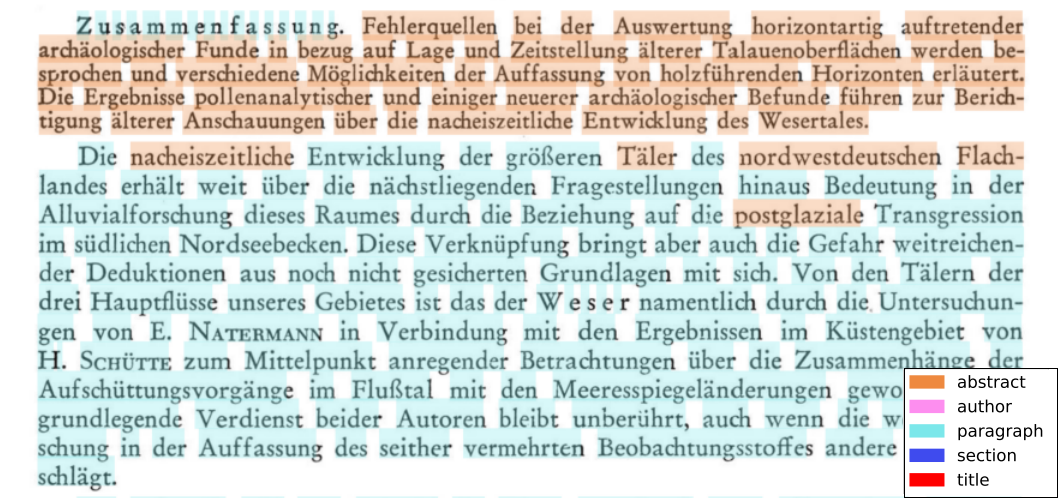
\includegraphics[width=0.8\linewidth]{images/no_seperation.png}
    \caption{An article with a less salient layout. Our model has a hard time predicting the end of the abstract section.}
    \label{fig:no_seperation}
\end{figure}
We also noticed better results on the DocBank portion of our created Document Segmentation dataset, as evident in Table~\ref{tab:results_docseg_lang}. We mainly attribute this to the overall homogeneity of the articles comprising the DocBank dataset, as these modern documents are created through the \LaTeX~typesetting system and mostly employ "streamlined" layouts and structure.\\
On the other hand, we have historic articles, which are far more diverse regarding structure and layout, for example articles beginning with an abstract followed by author and title, complicating the segmentation process.\\
References were even better detected by our model in the GEOcite portion of the dataset, suggesting that the internal text structure of reference strings might contribute more towards identification of references than visual information.\par
% reference parser
For the Reference Parser Model, we can also see a clear improvement of both transformer models against the CRF baseline model, as depicted in Table~\ref{tab:results_refseg_compare}. XLM-RoBERTa outperformed the fine-tuned mBERT model by a slight margin.\\
However, we encountered challenges while replicating the reported results for CRF models as documented by Boukhers et al.~\cite{excite_methods}. This discrepancy may indicate that the CRF model struggles with long-term dependencies in our reference segments, given that our dataset comprises reference segments instead of individual reference strings.\\
Despite facing a minor decrease in overall results following the implementation of our custom classification header and fine-tuning our model, both outputs still demonstrate favorable performance, as indicated in Figures~\ref{fig:results_final_refseg_cls} and~\ref{fig:results_final_refseg_ref}.\\
We further observed a difficulty in correctly classifying long URLs using our Reference Parser Model. Despite the expectation that the model would perform well on this class due to the fixed structure of URLs, we encountered challenges. We attribute this issue to the preprocessing of several special characters, which leads to the tokenization of URL sequences into long input sequences for our model. As a result, predicting them as a whole coherent class becomes challenging as showcased in Figure~\ref{fig:url_error}.

\begin{figure}[!t]
    \centering
    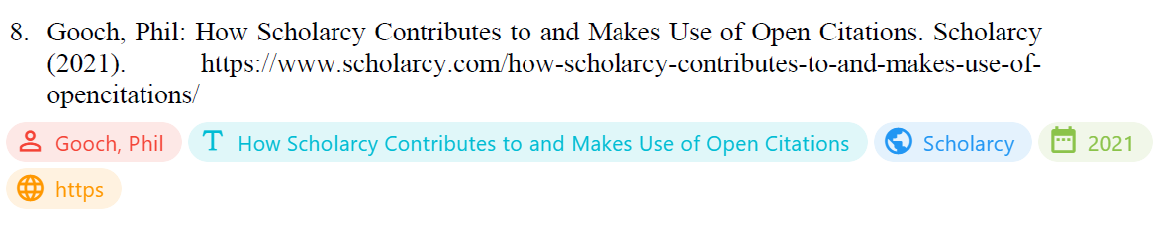
\includegraphics[width=1.0\linewidth]{images/url.png}
    \caption{An exemplary citation, where BiBEx was not able to extract the URL.}
    \label{fig:url_error}
\end{figure}

% author parser
The Author Parser Model showed similar results as the Document Segmentation Model and Reference Parser Model, where the CRF baseline model was outperformed by both transformer models, as indicated in Table~\ref{tab:results_author_comp}.\\
In our experiments, we used a cased version of XLM-RoBERTa since an uncased version, pretrained on a suitable corpus was not available at the time. Despite the expectation that the cased model might perform better, considering that upper case letters are strong indicators of a person's name, the fine-tuned mBERT model displayed better results than the XLM-RoBERTa model.\\
In general, we observed good results for all languages in our test set, with slightly lower performance for the English corpus compared to other languages, as shown in Table~\ref{tab:results_author_lang}.

\section{Extrinsic Evaluation}\label{sec:discussion_extrinsic}
As shown in Table~\ref{tab:results_overall_author}, the BiLSTM-CRF backend of GROBID performs worse than the CRF backend on our test corpus. This discrepancy might be due to various reasons such as differences in training data or an altered tokenization process. Further investigation and experimentation would be needed to determine the exact cause of this difference.\\
We observed that GROBID tends to extract tokens surrounding the title, leading to misclassifications such as labeling parts of the affiliation as authors. Additionally, it encounters difficulties when an article starts not directly at the top of a document page, especially if another article is present on the same page. These challenges may affect the overall performance of GROBID in our context, since the GEOcite corpus consists of various journals, where the end of an article and the start of another essay can be located on the same page.\\
In the case of BiBEx, we observed that the application often extracted correct author names, but faced challenges in accurately matching the actual author due to the limitations of our heuristics. These limitations can lead to wrongly split names, particularly in cases where the surname consists of multiple words, such as the nobiliary particles \enquote{af}, \enquote{von}, and \enquote{de}.\\
\begin{figure}[!ht]
    \centering
    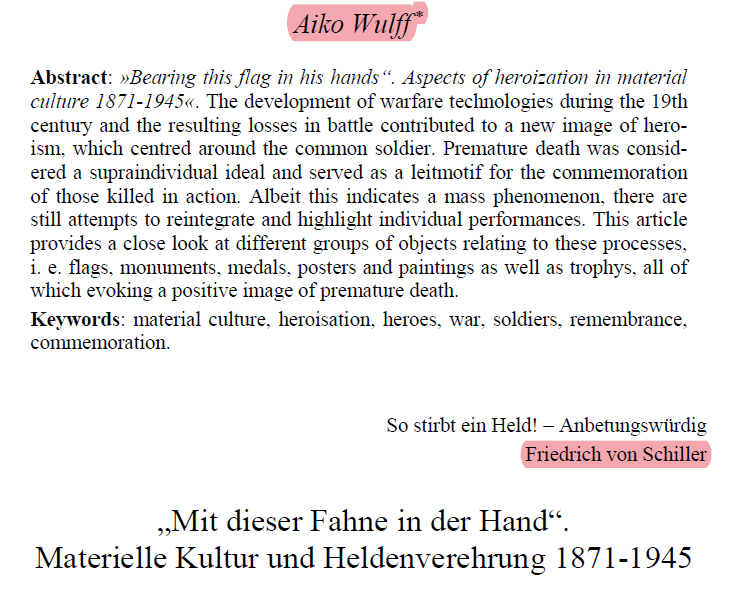
\includegraphics[width=0.6\linewidth]{images/bibex_author_wrong.png}
    \caption{BiBEx correctly predicts \enquote{Aiko Wulff}, but wrongly classifies \enquote{Friedrich von Schiller} as one of the authors of this article.}
    \label{fig:author_error}
\end{figure}
Furthermore, BiBEx occasionally misclassifies a person's name as an author, especially when they are in close proximity to the title. For instance, this can occur when an article is dedicated to a specific person, mentions editors, or displays a quote near the title, as seen in Figure~\ref{fig:author_error}.\\
During the reference extraction, as discussed in Section~\ref{sec:discussion_intrinsic}, BiBEx faces challenges when identifying URLs. Additionally, we observed that entities with long hyphenated sequences, such as titles, can occasionally be split into two or more entities of the same class.\\
On the positive side, our proposed system demonstrates effectiveness in distinguishing header sections of articles from citations, as illustrated in Figure~\ref{fig:ref_header}. This distinction is crucial, as it prevents falsely identified self-citations, a common occurrence with other tools.\\
As indicated in Table~\ref{tab:results_overall_author}, the BiBEx extraction application outperforms or achieves comparable results in most metrics for reference extraction. This is a promising outcome, indicating the effectiveness and robustness of our reference extraction approach.

\begin{figure}[!t]
    \centering
    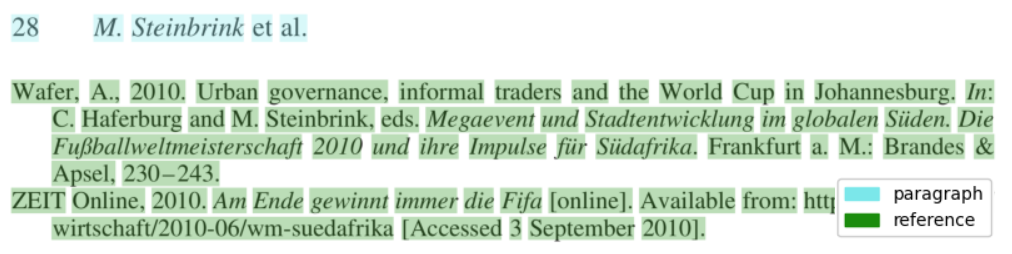
\includegraphics[width=0.9\linewidth]{images/header.png}
    \caption{BiBEx correctly classifies the header section of a page as paragraph, which could lead to false self-citations in a citation network, in case of a failure.}
    \label{fig:ref_header}
\end{figure}

\section{Limitations}\label{sec:discussion_limitations}

As described in our conceptual framework (Section~\ref{sec:conceptual_framework}), we intentionally limited the complexity of our BiBEx system to reduce potential errors stemming from upstream models. However, our findings indicate that the heuristics we employ to extract all parts of a name, may not comprehensively handle all possible name variations. To ensure accurate parsing of all author names, one option is to consider using a dedicated ML model instead of relying solely on heuristics. This would involve incorporating an additional layer of sequential models within our application. Alternatively, we could explore the use of diverse or adapted datasets, where names are already pre-segmented, allowing our current models to learn the correct name separation.\\
Additionally, we would like to emphasize the limited quantity of samples in datasets we utilized. Although more data is generally beneficial for machine learning models to enhance generalization and mitigate the impact of outliers, the availability of refined data tailored to our specific problem domain is sparse. Instead of prioritizing sheer quantity, our focus has been on annotating and utilizing datasets of the highest quality, meticulously tailored to address our specific challenges. This approach is evident in all datasets used for model training, intrinsic and extrinsic evaluation. For the extrinsic evaluation, it might be advantageous to have a slightly increased number of extracted authors and reference strings for testing purposes, providing a more definitive validation of our results.\\
However, another important aspect to consider is the composition of our Document Segmentation dataset. One part comprises mainly English, modern, machine-generated articles predominantly in STEM subjects, while the other part includes German, historical, scanned documents in the domain of Geography. To improve the generalization of our ML model, it would be beneficial to have a more homogenized dataset composition. This could involve augmenting the dataset with modern German articles or scanned historical documents written in English. By incorporating such variations, we believe our model would achieve an even better performance and adaptability across different types of publications.\\
Furthermore, we must highlight the limitations arising from our computational resources. Our usage of a Pro account for the cloud-based ML environment Google Colaboratory imposed constraints on the monthly GPU utilization. Large transformer models demand significant computational resources, even during the fine-tuning process. For instance, fine-tuning the LayoutXLM model on our training set for 2 epochs, using a v100 GPU, took approximately one hour, accounting for roughly 5\% of our monthly quota. Consequently, this limitation impacted the number of hyperparameters we could explore and the maximum number of transformer models we could test, leading to some constraints in our experimental setup.